% Generated mechanically from the reviewed Markdown source.
% Controller edits should be made in both source and LaTeX when material.

\section{ThreadBench}

\subsection{Process–Artifact Evaluation}

A polished deck can conceal a broken handoff: research evidence may never reach the plan, a planned image may never be used, or a rendered defect may never be repaired. Final-only scores see the artifact but cannot locate the broken transfer. ThreadBench therefore evaluates case-specific process evidence separately from the delivered deck. It is process-aware and artifact-grounded; it does not claim coverage of every engineering stage.

\begin{figure}[H]
\centering
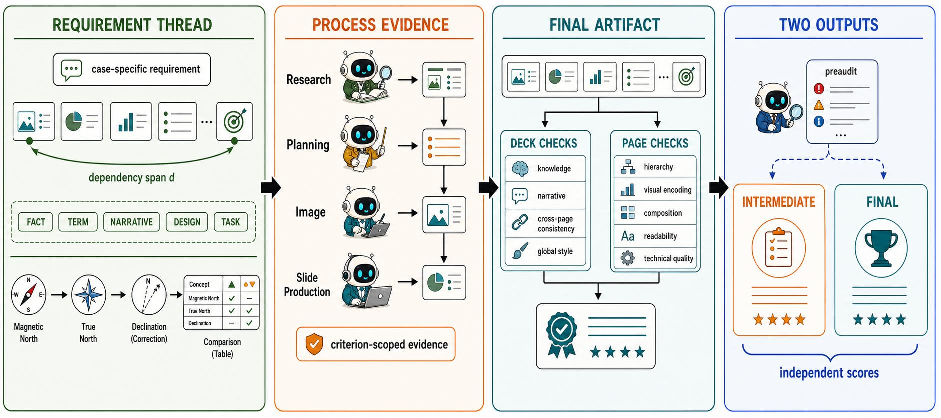
\includegraphics[width=\linewidth]{figures/fig4_threadbench_anatomy.pdf}
\caption{\textbf{Anatomy of ThreadBench.} A case-specific requirement defines an observable source-to-target closure rule across a deck. Intermediate evaluation follows anchored evidence through Research, Planning, Image, and Slide Production, whereas Final evaluation inspects the canonical rendered deck at deck and page granularity. The two layers produce independent scores rather than a single blended metric. The animal-navigation thread is the current formal reference case.}
\label{fig:threadbench-anatomy}
\end{figure}

\subsection{Requirement Threads and the Two-Layer Rubric}

Figure~\ref{fig:threadbench-anatomy} makes the evaluation unit explicit. A requirement thread starts from a source requirement or anchor, specifies a distant target and an observable closure rule, and may encode factual, terminological, narrative, design, or task-level dependence. The Intermediate layer evaluates seven criterion families across Research, Planning, Image, and Slide Production, using criterion-scoped packets that expose only relevant anchored evidence. The Final layer evaluates the canonical artifact in two groups: Deck combines a Knowledge checklist with six whole-deck dimensions, while Page scores five visual and technical dimensions for every canonical page. The complete criterion inventory and dimension definitions are in Appendix~\ref{app:protocol}.

\subsection{Scoring and Release Boundary}

The Judge first matches evidence to explicit anchors; code then derives 0/0.5/1 scores (Knowledge is binary). Deck and Page each receive one weakest-dimension decay, whereas Intermediate does not:

\[
G_{\mathrm{eff}}=G_{\mathrm{base}}[1-0.3(1-G_{\min})],\quad
F=\tfrac12(Deck_{\mathrm{eff}}+Page_{\mathrm{eff}}),\quad
I=\operatorname{mean}(R,P,I_m,S).
\]

where \(I_m\) denotes the Image dimension and only applicable Intermediate dimensions enter the mean. The released Intermediate \(I\) and Final \(F\) fields remain independent and are never collapsed into one scalar. The executable v004 contract currently specifies one formal reference case (\url{Education/Education-lh-Animal_navigation}). Appendix~\ref{app:protocol} gives the N/A semantics, major-defect deductions, optional non-scoring Preaudit, and human–Judge calibration; multi-domain expansion and explicit span diagnostics remain outside the current release.

\section{Experiments}

We organize experiments around four research questions. \textbf{RQ1 (general quality):} How good are the complete decks that MuralPresenter produces under general-quality evaluation? \textbf{RQ2 (multi-turn revision):} Without dedicated editing training, can it perform multi-turn edits? \textbf{RQ3 (process–artifact consistency):} Does the production chain preserve requirements and evidence through intermediate stages and into the final deck? \textbf{RQ4 (design choices):} How much do the delegation boundary, responsibility topology, two-level visual critique, and trajectory supervision each contribute?

\subsection{Setup}

\textbf{MuralPresenter-9B.} We use DeepSeek-V4-Flash as the rollout backbone and Gemini-3.5-Flash as the visual critic, sampling trajectories over \resulttbd{[TBD:9B\_TASKS]} training tasks (§4). Quality filtering retains exactly 1,000 post-QC trajectories. We fine-tune Qwen-3.5-9B with MS-SWIFT~\citep{zhao2024mswift} for \resulttbd{[TBD:9B\_EPOCH]} epochs, global batch 32, LR \(1\times10^{-5}\), and context length \resulttbd{[TBD:9B\_CTX]}, using \resulttbd{[TBD:9B\_GPU]} A800 GPUs for \resulttbd{[TBD:9B\_GPUH]} GPU-hours.

\textbf{Data and training (verified 27B).} MuralPresenter-27B uses the proprietary-teacher trajectory cohort described in §4: 293{,}436 base trajectories become 318{,}422 training exposures (\textasciitilde7.31B content tokens; \textasciitilde56{,}458 packed 128K sequences) after resampling and length filtering. We perform full-parameter SFT on Qwen-3.5-27B via the Megatron backend of MS-SWIFT: 128K context, 1 epoch, global batch 32, LR \(2\times10^{-5}\) with cosine decay to \(1\times10^{-6}\) after 5\% warmup, on 32 80GB GPUs (4 nodes, TP=4, CP=2, DP=4, micro-batch 1, gradient accumulation 8); the vision encoder and modality aligner are frozen. Training runs 1{,}764 steps in \textasciitilde50.3 hours (\textasciitilde1{,}604 GPU-hours). Gemini-3.5-Flash serves only as the QC-stage quality scorer. The full data/model ledger is in Appendix~\ref{app:protocol}.

\textbf{Baselines.} ThreadBench retains six strong general-purpose controls: Opus-4.7, Sonnet-5, GPT-5.6-luna, Gemini-3.5-Flash, Qwen-3.7-plus, and Kimi-k3. Existing-benchmark reruns use a compact five-system cohort: the 9B synthesis pipeline (DeepSeek-V4-Flash + Gemini-3.5-Flash), untuned Qwen-3.5-9B and Qwen-3.6-27B controls, and our 9B and 27B models. All five share the same benchmark inputs and adapter. To expose absolute position on each external benchmark, Tables~\ref{tab:general}--\ref{tab:edit} also include selected leading systems from the original papers in a separate \emph{reported} block. These values retain their source protocols, are not our reruns, and are never pooled with the unified cohort or entered into significance tests; complete reported tables appear in Appendix~\ref{app:protocol}.

\textbf{Interpretation boundary.} The 9B and 27B checkpoints differ in teacher provenance, corpus scale, base model, and training recipe. We report both as system variants but do not interpret their difference as a controlled scaling or data-efficiency result. We conduct RQ4 ablations in the 9B setting with the same 1K corpus and fixed training variables. Comparisons against proprietary frontier controls on ThreadBench are end-to-end system comparisons and do not establish teacher-independent generalization.

\textbf{Metric contracts.} PresentBench~\citep{chen2026presentbench} and SlidesGen-Bench~\citep{yang2026slidesgenbench} measure general quality, DECKBench~\citep{jang2026deckbench} measures multi-turn revision, and ThreadBench (§5) measures process–artifact consistency via separate Intermediate and Final scores with dimension-level diagnostics. Bounded quality, similarity, success, and ThreadBench scores are interpreted as higher-is-better; SlidesGen-Bench PEI remains an ordinal editability level, while signed DECKBench change metrics retain the official protocol's direction and are not merged with absolute quality scores. We freeze the official metric versions, direction, aggregation code, and hashes for all runs. Full dimensions and secondary diagnostics are in Appendix~\ref{app:protocol}.

\subsection{Main Results}

\textbf{General generation quality (RQ1).} Table~\ref{tab:general} places the five-system rerun cohort beside selected original-paper leaders on PresentBench Overall and SlidesGen-Bench Content, Aesthetics, and Editability (PEI). Full sub-dimensions and reported systems are in Appendix~\ref{app:protocol}. This table addresses general deck quality and draws no conclusion about long-horizon consistency.

\begin{table}[!htbp]
\centering
\small
\caption{RQ1: selected original-paper leaders (reported under source protocols) and our five-system unified reruns on PresentBench and SlidesGen-Bench. Full reported systems and dimensions are in Appendix~\ref{app:protocol}.}
\label{tab:general}
\begingroup
\let\texttt\resulttbd
\setlength{\tabcolsep}{4pt}
\begin{tabularx}{\linewidth}{@{}>{\raggedright\arraybackslash}Xcccc@{}}
\toprule
& PresentBench & \multicolumn{3}{c}{SlidesGen-Bench} \\
\cmidrule(lr){2-2}\cmidrule(lr){3-5}
System & Overall & Content & Aesthetics & Editability (PEI) \\
\midrule
\multicolumn{5}{l}{\emph{Original-paper references (reported)}} \\
NotebookLM       & 62.5 & 74.21 & 22.82 & L0 \\
Zhipu            & ---  & 88.29 & 22.06 & L2 \\
Skywork-Banana   & ---  & 83.83 & 27.28 & L1 \\
Quark            & ---  & 81.40 & 16.86 & L3 \\
\midrule
\multicolumn{5}{l}{\emph{Unified reruns (same inputs and adapter)}} \\
9B synth. pipeline (DS-V4 + Gemini-3.5) & \resulttbd{[TBD:G\_TC\_PB]} & \resulttbd{[TBD:G\_TC\_SGC]} & \resulttbd{[TBD:G\_TC\_SGA]} & \resulttbd{[TBD:G\_TC\_SGE]} \\
Qwen-3.5-9B (untuned)  & \resulttbd{[TBD:G\_Q9\_PB]}  & \resulttbd{[TBD:G\_Q9\_SGC]}  & \resulttbd{[TBD:G\_Q9\_SGA]}  & \resulttbd{[TBD:G\_Q9\_SGE]} \\
Qwen-3.6-27B (untuned) & \resulttbd{[TBD:G\_Q27\_PB]} & \resulttbd{[TBD:G\_Q27\_SGC]} & \resulttbd{[TBD:G\_Q27\_SGA]} & \resulttbd{[TBD:G\_Q27\_SGE]} \\
MuralPresenter-9B  & \resulttbd{[TBD:G\_M9\_PB]}  & \resulttbd{[TBD:G\_M9\_SGC]}  & \resulttbd{[TBD:G\_M9\_SGA]}  & \resulttbd{[TBD:G\_M9\_SGE]} \\
MuralPresenter-27B & \resulttbd{[TBD:G\_M27\_PB]} & \resulttbd{[TBD:G\_M27\_SGC]} & \resulttbd{[TBD:G\_M27\_SGA]} & \resulttbd{[TBD:G\_M27\_SGE]} \\
\bottomrule
\end{tabularx}
\endgroup
\end{table}

The reported block anchors the published frontier at 62.5 PresentBench Overall (NotebookLM), 88.29 Content (Zhipu), 27.28 Aesthetics (Skywork-Banana), and PEI L3 (Quark). MuralPresenter-9B reaches \resulttbd{[TBD:G\_M9\_PB]} PresentBench Overall and MuralPresenter-27B reaches \resulttbd{[TBD:G\_M27\_PB]}, compared with \resulttbd{[TBD:G\_BEST\_CONTROL\_PB]} for the strongest unified-rerun control. On SlidesGen-Bench, the two models obtain Content/Aesthetics/PEI triples of \resulttbd{[TBD:G\_M9\_TRIPLE]} and \resulttbd{[TBD:G\_M27\_TRIPLE]}. Relative to the reported frontier, \resulttbd{[TBD:G\_REPORTED\_COMPARISON]}; within the controlled rerun cohort, the results indicate \resulttbd{[TBD:G\_RQ1\_INTERPRETATION]}. Neither comparison is used to infer long-horizon consistency.

\textbf{Multi-turn revision (RQ2).} Table~\ref{tab:edit} places the same five rerun systems beside selected DECKBench configurations reporting Deck Fidelity, Layout Quality, Transition Similarity, \(\Delta\)-DTW, and \(\Delta\)-Transition Similarity. PPT-Eval~\citep{gandhi2026ppteval} remains a supplementary transfer test and includes its reported leading reference. Complete original-paper fields are in Appendix~\ref{app:protocol}. Transfer from inspect--diagnose--patch behavior is one hypothesis tested by RQ4.

\begin{table}[!htbp]
\centering
\footnotesize
\caption{RQ2: selected original-paper DECKBench references and our five-system unified reruns; PPT-Eval is supplementary and remains a separate protocol. Full reported fields are in Appendix~\ref{app:protocol}.}
\label{tab:edit}
\begingroup
\let\texttt\resulttbd
\setlength{\tabcolsep}{3pt}
\begin{tabularx}{\linewidth}{@{}>{\raggedright\arraybackslash}Xccccc@{}}
\toprule
& Deck & Slide & Deck & \multicolumn{2}{c}{Multi-turn} \\
\cmidrule(lr){2-2}\cmidrule(lr){3-3}\cmidrule(lr){4-4}\cmidrule(lr){5-6}
System & Fidelity & Layout Q. & Trans.\ Sim. & \(\Delta\)-DTW & \(\Delta\)-Trans.\ Sim. \\
\midrule
\multicolumn{6}{l}{\emph{Original-paper references (reported)}} \\
Auto-Slides (GPT-4o) & 0.591 & 0.998 & 0.858 & --- & --- \\
DECKBench (GPT-4o)   & 0.584 & 1.000 & 0.879 & --- & --- \\
GPT-5.1 sim. + GPT-5-mini edit. (High) & --- & --- & --- & 0.02278 & 0.03230 \\
Kimi K2 sim. + DeepSeek edit. (High)   & --- & --- & --- & 0.01549 & 0.04287 \\
\midrule
\multicolumn{6}{l}{\emph{Unified reruns (same inputs and adapter)}} \\
9B synth. pipeline (DS-V4 + Gemini-3.5) & \resulttbd{[TBD:E\_TC\_DFID]} & \resulttbd{[TBD:E\_TC\_SLQ]} & \resulttbd{[TBD:E\_TC\_DTSIM]} & \resulttbd{[TBD:E\_TC\_MDDTW]} & \resulttbd{[TBD:E\_TC\_MDTS]} \\
Qwen-3.5-9B (untuned)  & \resulttbd{[TBD:E\_Q9\_DFID]}  & \resulttbd{[TBD:E\_Q9\_SLQ]}  & \resulttbd{[TBD:E\_Q9\_DTSIM]}  & \resulttbd{[TBD:E\_Q9\_MDDTW]}  & \resulttbd{[TBD:E\_Q9\_MDTS]} \\
Qwen-3.6-27B (untuned) & \resulttbd{[TBD:E\_Q27\_DFID]} & \resulttbd{[TBD:E\_Q27\_SLQ]} & \resulttbd{[TBD:E\_Q27\_DTSIM]} & \resulttbd{[TBD:E\_Q27\_MDDTW]} & \resulttbd{[TBD:E\_Q27\_MDTS]} \\
MuralPresenter-9B  & \resulttbd{[TBD:E\_M9\_DFID]}  & \resulttbd{[TBD:E\_M9\_SLQ]}  & \resulttbd{[TBD:E\_M9\_DTSIM]}  & \resulttbd{[TBD:E\_M9\_MDDTW]}  & \resulttbd{[TBD:E\_M9\_MDTS]} \\
MuralPresenter-27B & \resulttbd{[TBD:E\_M27\_DFID]} & \resulttbd{[TBD:E\_M27\_SLQ]} & \resulttbd{[TBD:E\_M27\_DTSIM]} & \resulttbd{[TBD:E\_M27\_MDDTW]} & \resulttbd{[TBD:E\_M27\_MDTS]} \\
\midrule
\multicolumn{6}{l}{\emph{PPT-Eval (supplementary, official protocol, not comparable to the above)}} \\
& \multicolumn{2}{c}{Success Rate} & \multicolumn{3}{c}{Avg.\ Partial Score} \\
Claude-4.5-Opus (reported) & \multicolumn{2}{c}{45\%} & \multicolumn{3}{c}{57\%} \\
MuralPresenter-27B & \multicolumn{2}{c}{\resulttbd{[TBD:E\_M27\_PESR]}} & \multicolumn{3}{c}{\resulttbd{[TBD:E\_M27\_PEPS]}} \\
\bottomrule
\end{tabularx}
\endgroup
\end{table}

The reported DECKBench block exposes the published range without constructing a fictitious composite baseline: Auto-Slides leads the displayed Fidelity value, DECKBench (GPT-4o) leads Layout and Transition Similarity, and the two high-granularity simulator/editor configurations provide the multi-turn references. Across unified reruns, MuralPresenter-9B changes Deck Fidelity and Layout Quality by \resulttbd{[TBD:E\_M9\_SUMMARY]} relative to untuned Qwen-3.5-9B, while MuralPresenter-27B changes them by \resulttbd{[TBD:E\_M27\_SUMMARY]} relative to its 27B control. The multi-turn deltas show \resulttbd{[TBD:E\_MULTITURN\_INTERPRETATION]}; relative to reported external references, \resulttbd{[TBD:E\_REPORTED\_COMPARISON]}. PPT-Eval yields \resulttbd{[TBD:E\_PPTEVAL\_INTERPRETATION]} against the reported 45\%/57\% Claude-4.5-Opus reference. Together with RQ4, this supports \resulttbd{[TBD:E\_RQ2\_CONCLUSION]} about transfer from inspect--diagnose--patch supervision.

\textbf{Process–artifact consistency (RQ3).} Table~\ref{tab:thread} reports ThreadBench Intermediate and Final scores along with interpretable group breakdowns (Deck and Page effective scores). These are the two independent outputs of the v004 scoring contract (§5.3). Dimension-level diagnostics for all systems are in Appendix~\ref{app:protocol}.

\begin{table}[!htbp]
\centering
\small
\caption{RQ3: ThreadBench process–artifact consistency. Intermediate and Final are independent 0–1 scores; Deck and Page are the two Final sub-groups after weakest-dimension decay.}
\label{tab:thread}
\begingroup
\let\texttt\resulttbd
\setlength{\tabcolsep}{5pt}
\begin{tabularx}{\linewidth}{@{}>{\raggedright\arraybackslash}Xcccc@{}}
\toprule
& \multicolumn{1}{c}{Intermediate} & \multicolumn{3}{c}{Final} \\
\cmidrule(lr){2-2}\cmidrule(lr){3-5}
System & Score & Score & Deck\(_{eff}\) & Page\(_{eff}\) \\
\midrule
Opus-4.7            & \resulttbd{[TBD:T\_OP\_INT]}  & \resulttbd{[TBD:T\_OP\_FIN]}  & \resulttbd{[TBD:T\_OP\_DECK]} & \resulttbd{[TBD:T\_OP\_PAGE]} \\
Sonnet-5            & \resulttbd{[TBD:T\_SN\_INT]}  & \resulttbd{[TBD:T\_SN\_FIN]}  & \resulttbd{[TBD:T\_SN\_DECK]} & \resulttbd{[TBD:T\_SN\_PAGE]} \\
GPT-5.6-luna        & \resulttbd{[TBD:T\_LU\_INT]}  & \resulttbd{[TBD:T\_LU\_FIN]}  & \resulttbd{[TBD:T\_LU\_DECK]} & \resulttbd{[TBD:T\_LU\_PAGE]} \\
Gemini-3.5-Flash    & \resulttbd{[TBD:T\_GM\_INT]}  & \resulttbd{[TBD:T\_GM\_FIN]}  & \resulttbd{[TBD:T\_GM\_DECK]} & \resulttbd{[TBD:T\_GM\_PAGE]} \\
Qwen-3.7-plus       & \resulttbd{[TBD:T\_QW\_INT]}  & \resulttbd{[TBD:T\_QW\_FIN]}  & \resulttbd{[TBD:T\_QW\_DECK]} & \resulttbd{[TBD:T\_QW\_PAGE]} \\
Kimi-k3             & \resulttbd{[TBD:T\_KM\_INT]}  & \resulttbd{[TBD:T\_KM\_FIN]}  & \resulttbd{[TBD:T\_KM\_DECK]} & \resulttbd{[TBD:T\_KM\_PAGE]} \\
\midrule
MuralPresenter-9B  & \resulttbd{[TBD:T\_M9\_INT]}  & \resulttbd{[TBD:T\_M9\_FIN]}  & \resulttbd{[TBD:T\_M9\_DECK]} & \resulttbd{[TBD:T\_M9\_PAGE]} \\
MuralPresenter-27B & \resulttbd{[TBD:T\_M27\_INT]} & \resulttbd{[TBD:T\_M27\_FIN]} & \resulttbd{[TBD:T\_M27\_DECK]} & \resulttbd{[TBD:T\_M27\_PAGE]} \\
\bottomrule
\end{tabularx}
\endgroup
\end{table}

MuralPresenter-9B obtains \resulttbd{[TBD:T\_M9\_INT]}/\resulttbd{[TBD:T\_M9\_FIN]} Intermediate/Final, and MuralPresenter-27B obtains \resulttbd{[TBD:T\_M27\_INT]}/\resulttbd{[TBD:T\_M27\_FIN]}. Relative to the strongest general-purpose baseline, the corresponding differences are \resulttbd{[TBD:T\_M9\_DELTA]} and \resulttbd{[TBD:T\_M27\_DELTA]}. The Deck/Page split reveals \resulttbd{[TBD:T\_RQ3\_INTERPRETATION]}, showing whether the dominant bottleneck lies in requirement transfer or rendered-page quality.

\subsection{Ablation (RQ4)}

Table~\ref{tab:ablation} reports four one-factor-at-a-time ablations against one shared Full reference in the 9B setting, using the same 1K training corpus and holding all other training variables fixed. \textbf{Delegation boundary:} single-context or always-delegate. \textbf{Responsibility topology:} per-slide or fixed-adjacent grouping; this isolates whether dependency-aligned grouping contributes beyond generic decomposition. \textbf{Two-level visual critique:} removing group-level or whole-deck review individually. \textbf{Trajectory supervision:} output-only SFT or removing inspect--diagnose--patch steps. Primary scores are ThreadBench Intermediate and Final; the cross-page semantic-consistency dimension provides a topology-sensitive diagnostic.

\begin{table}[!htbp]
\centering
\footnotesize
\caption{RQ4 controlled ablations against one shared Full reference. Intermediate and Final are aggregate outputs; Cross-page is the Final Deck semantic-consistency dimension.}
\label{tab:ablation}
\begingroup
\let\texttt\resulttbd
\setlength{\tabcolsep}{3pt}
\begin{tabularx}{\linewidth}{@{}>{\raggedright\arraybackslash}p{0.19\linewidth}>{\raggedright\arraybackslash}Xccc@{}}
\toprule
Factor & Variant & Intermediate & Final & Cross-page \\
\midrule
Full reference (ours) & on-demand + dep.-aligned + both critique + full traj. & \resulttbd{[TBD:A\_FULL\_INT]} & \resulttbd{[TBD:A\_FULL\_FIN]} & \resulttbd{[TBD:A\_FULL\_XSEM]} \\
\midrule
Delegation boundary & Single-context      & \resulttbd{[TBD:A\_DEL\_SC\_INT]}  & \resulttbd{[TBD:A\_DEL\_SC\_FIN]} & \resulttbd{[TBD:A\_DEL\_SC\_XSEM]} \\
                    & Always-delegate     & \resulttbd{[TBD:A\_DEL\_AD\_INT]}  & \resulttbd{[TBD:A\_DEL\_AD\_FIN]} & \resulttbd{[TBD:A\_DEL\_AD\_XSEM]} \\
\midrule
Responsibility topology & Per-slide ownership & \resulttbd{[TBD:A\_TOP\_PS\_INT]}  & \resulttbd{[TBD:A\_TOP\_PS\_FIN]} & \resulttbd{[TBD:A\_TOP\_PS\_XSEM]} \\
                    & Fixed-adjacent      & \resulttbd{[TBD:A\_TOP\_FA\_INT]}  & \resulttbd{[TBD:A\_TOP\_FA\_FIN]} & \resulttbd{[TBD:A\_TOP\_FA\_XSEM]} \\
\midrule
Two-level visual critique & w/o group-level     & \resulttbd{[TBD:A\_VIS\_NG\_INT]}  & \resulttbd{[TBD:A\_VIS\_NG\_FIN]} & \resulttbd{[TBD:A\_VIS\_NG\_XSEM]} \\
                    & w/o whole-deck      & \resulttbd{[TBD:A\_VIS\_NW\_INT]}  & \resulttbd{[TBD:A\_VIS\_NW\_FIN]} & \resulttbd{[TBD:A\_VIS\_NW\_XSEM]} \\
\midrule
Trajectory supervision & Output-only SFT     & \resulttbd{[TBD:A\_SUP\_OO\_INT]}  & \resulttbd{[TBD:A\_SUP\_OO\_FIN]} & \resulttbd{[TBD:A\_SUP\_OO\_XSEM]} \\
                    & w/o inspect--patch  & \resulttbd{[TBD:A\_SUP\_NI\_INT]}  & \resulttbd{[TBD:A\_SUP\_NI\_FIN]} & \resulttbd{[TBD:A\_SUP\_NI\_XSEM]} \\
\bottomrule
\end{tabularx}
\endgroup
\end{table}

Replacing dependency-aligned groups with per-slide or fixed-adjacent ownership changes Cross-page consistency by \resulttbd{[TBD:A\_TOPOLOGY\_EFFECT]}; changing the delegation boundary changes Final by \resulttbd{[TBD:A\_DELEGATION\_EFFECT]}. Removing group- or deck-level critique yields \resulttbd{[TBD:A\_CRITIQUE\_EFFECT]}, while output-only and no-inspect supervision yield \resulttbd{[TBD:A\_SUPERVISION\_EFFECT]}. The combined pattern yields \resulttbd{[TBD:A\_RQ4\_INTERPRETATION]}, separating the responsibility-topology effect from generic multi-Agent decomposition.
